\documentclass[11pt,a4paper,twoside,french,svgnames]{report}
\usepackage[utf8]{inputenc} % force the use of utf8
\usepackage[T1]{fontenc} % font encoding, allows accents
\usepackage[papersize={21cm,29.7cm},top= 2.5cm,bottom=2.5cm, inner=2.5cm, outer=2.5cm]{geometry} % page formatting
\usepackage[francais]{babel} % translate everything in the desired language: table of contents, etc. 'english' can be replaced with 'francais'
\usepackage{graphicx} % images management
\usepackage{wrapfig} % floating images
\usepackage{array} % allow arrays
\usepackage{fancyhdr} % headers/footers management (overrides empty, plain and headings)
\usepackage{listings} % code insertion (MUST BE WRITTEN AFTER BABEL)
%\usepackage[nottoc,numbib]{tocbibind} % bib in toc
%\usepackage{pdfpages} % include PDF documents
\usepackage{enumitem} % for /setlist
\usepackage{color,soul} % add some colors and hightlight
\usepackage{xcolor} % more colors
\usepackage[hyphens]{url} % auto break lines in URL
\usepackage[hidelinks,  colorlinks  = true, % no borders, colors enabled
                        anchorcolor = blue,
                        linkcolor   = black, % links in table of contents
                        urlcolor    = blue,
                        citecolor   = blue]{hyperref}
%\usepackage[%nonumberlist,% no page number
%            toc,% displayed in toc
%            numberedsection,% displayed as a numbered section in toc
%            xindy]{glossaries} % glossary with xindy style. MUST BE WRITTEN AFTER HYPERREF
%\setglossarystyle{listgroup}

\sethlcolor{cyan} % package soul
\newcommand{\file}[1]{\hl{\emph{#1}}} % highlight a file URI

%\makeglossaries
%\loadglsentries{glossary.tex}

%%%%%%%%%%%%%%%%%%%%%%%%%%%%%%%%%%%%%%%%%%%%%%%%%%%%%%%% LISTINGS %%%%%%%%%%%%%%%%%%%%%%%%%%%%%%%%%%%%%%%%%%%%%%%%%%%%%%%%
\definecolor{comment}{rgb}{0.12, 0.38, 0.18 } % adjusted, in Eclipse: {0.25, 0.42, 0.30 } = #3F6A4D
\definecolor{keyword}{rgb}{0.37, 0.08, 0.25}  % #5F1441
\definecolor{string}{rgb}{0.06, 0.10, 0.98} % #101AF9

\lstset{
  columns=flexible, %prevent extra spaces
  rulecolor=\color{black!50},
  backgroundcolor = \color{blue!10},
  numbers=none, % line numbering
  showspaces=false,
  showtabs=false,
  tabsize=4,
  breaklines=true,
  showstringspaces=false,
  breakatwhitespace=false,
  commentstyle=\color{comment},
  keywordstyle=\color{keyword},
  stringstyle=\color{string},
  basicstyle=\ttfamily,
  extendedchars=true,
  emph=[2]{In},
  emphstyle=[2]\color{black!70},
  morecomment=[l][\color{blue}]{Out},
  frame=single,
  frameround=tttt,
  framerule=0.3pt,
  framesep=4pt,
  belowcaptionskip=2.1pt,
  literate={à}{{\`a }}1 {â}{{\^a}}1 %                         letter a
           {À}{{\`A}}1 {Â}{{\^A}}1 %                         letter A
           {ç}{{\c{c}}}1 %                                   letter c
           {Ç}{{\c{C}}}1 %                                   letter C
           {é}{{\'e}}1 {è}{{\`e}}1 {ê}{{\^e}}1 {ë}{{\"e}}1 % letter e
           {É}{{\'E}}1 {È}{{\`E}}1 {Ê}{{\^E}}1 {Ë}{{\"E}}1 % letter E
           {î}{{\^i}}1 {ï}{{\"i}}1 %                         letter i
           {Î}{{\^I}}1 {Ï}{{\"I}}1 %                         letter I
           {ô}{{\^o}}1 %                                     letter o
           {Ô}{{\^O}}1 %                                     letter O
           {œ}{{\oe}}1 %                                     letter oe
           {Œ}{{\OE}}1 %                                     letter OE
           {ù}{{\`u}}1 {û}{{\^u}}1 {ü}{{\"u}}1 %             letter u
           {Ù}{{\`U}}1 {Û}{{\^U}}1 {Ü}{{\"U}}1 %             letter U
  % above is a hack to force UTF8 compatibility (only for french)
}

\newcommand{\textcode}[1]{\lstset{
  title={{\setlength{\fboxsep}{1pt}\fcolorbox{orange}{yellow!20}{\sffamily\scriptsize
              \textcolor{gray!10}{\_}{#1}\textcolor{gray!10}{\_}}}}
  }
}

\newcommand{\clanguage}{\lstset{
  language=C,
  title={{\setlength{\fboxsep}{1pt}\fcolorbox{orange}{yellow!20}{\sffamily\scriptsize
              \textcolor{gray!10}{\_}C\textcolor{gray!10}{\_}}}}
  }
}
%%%%%%%%%%%%%%%%%%%%%%%%%%%%%%%%%%%%%%%%%%%%%%%%%%%%%%%%%%%%%%%%%%%%%%%%%%%%%%%%%%%%%%%%%%%%%%%%%%%%%%%%%%%%%%%%%%%%%%%%%%%

%\parindent=20pt
\fancypagestyle{plain}{
    % Headers
    \fancyhead[R]{Rapport TD5 SR02}
    \fancyhead[L]{Anaïs \textsc{NEVEUX} - Romain \textsc{PELLERIN}}

    % Footers
    \renewcommand{\footrulewidth}{0.1pt}
    \fancyfoot[C]{Université de Technologie de Compiègne}
    \fancyfoot[LE]{\ifnum\thepage>0 \thepage \fi}
    \fancyfoot[RO]{\ifnum\thepage>0 \thepage \fi}
}

\fancypagestyle{empty}{%
    \renewcommand{\headrulewidth}{0pt} % No sub line
    \fancyhead{} % Empty the header

    \renewcommand{\footrulewidth}{0pt}
    \fancyfoot{}
} 

\setlist[itemize,2]{label={$\bullet$}} % use bullets for nested itemize

% First page
\newcommand{\presentation}[1]{\vspace{0.3cm}\large{\textbf{#1}}\vspace{0.3cm}\\}
\newcommand{\presentationLarge}[1]{\vspace{0.3cm}\LARGE{\textbf{#1}}\vspace{0.3cm}\\}

% Overrides chapter (numbered and no-numbered) headings: remove space, display only the title
\makeatletter
  \def\@makechapterhead#1{%
  \vspace*{0\p@}% avant 50
  {\parindent \z@ \raggedright \normalfont
    %\ifnum \c@secnumdepth >\m@ne
    %    \huge\bfseries \@chapapp\space \thechapter
    %    \par\nobreak
    %    \vskip 20\p@
    %\fi
    \interlinepenalty\@M
    \Huge \bfseries \thechapter\quad #1   
    \vskip 40\p@
  }}
  \def\@makeschapterhead#1{%
  \vspace*{0\p@}% before 50
  {\parindent \z@ \raggedright
    \normalfont
    \interlinepenalty\@M
    \Huge \bfseries  #1\par\nobreak
    \vskip 40\p@
  }}
\makeatother

\newcommand{\ignore}[1]{} % inline comments

\pagenumbering{arabic}
%\addtocounter{page}{-7} % page numbering starts at 1 + (-7)
\pagestyle{plain} % uses fancy

\title{Rapport SR02}
\author{Anaïs NEVEUX et Romain PELLERIN}
\date\today

%\setcounter{tocdepth}{4}

\begin{document}
\thispagestyle{empty} % only for the current page

\begin{center}

\includegraphics[height=3cm]{UTC_logo.png}\\
\vspace{2.5cm}
\presentation{Université de Technologie de Compiègne} 
\presentation{SR02}

\vspace{2cm}
\noindent\fbox{
\begin{minipage}{0.9\textwidth}
\begin{center}
    \presentationLarge{Rapport de TD}
    \presentationLarge{\Huge{5 - Librairie de sémaphores}}
\end{center}
\end{minipage}}
\vspace{3cm}

\presentation{Printemps 2015}
\vspace{1cm}

\def\arraystretch{1.5} % 1 is the default
\begin{tabular}{|>{\hfill\arraybackslash}p{5cm}|p{5cm}|}
\hline
    \multicolumn{2}{|c|}{Anaïs \textsc{NEVEUX} - Romain \textsc{PELLERIN}}\\
\hline
     \multicolumn{2}{|c|}{Groupe 2}\\% dates
\hline
    \multicolumn{2}{|c|}{\textit{\today}}\\% dates
\hline
\end{tabular}
\end{center}

\tableofcontents

\part{Séance 1}
\clanguage

\chapter{Création d'une bibliothèque P(), V()}

\section{Question 1}

\subsection{\lstinline{int init\_semaphore(void)}}

Le but de cette fonction est de créer un ensemble de \lstinline{N_SEM} sémaphores, qui pourront être utilisés dans le cadre de processus père-fils (suite à un \lstinline{fork()}) uniquement, à cause de l'utilisation d'\lstinline{IPC_PRIVATE} comme clé lors de la création. Dans le cas où notre \lstinline{semid}, représentant notre groupement, ne vaut ni -2 (aucune création), ou -1 (erreur lors d'une précédente création), on retourne -1. Dans le cas d'une erreur lors de la création, un message d'erreur est envoyé et on retourne -2.
Dans les autres cas, on instancie une variable de type \lstinline{union semun} qui servira à l'initialisation des sémaphores grâce au flag SETALL. On retourne 0.

\textcode{sem\_pv.c}
\begin{lstlisting}
int init_semaphore(void) {
    if (semid != -2 && semid != -1) {
        fprintf(stderr, "Déjà créé.\n");
        return -1; // Erreur récupérable avec errno
    }
    else if((semid = semget(IPC_PRIVATE, N_SEM, 0666)) == -1) { // crée un ou des sémaphores, alternative : semget(CLE, N_SEM, IPC_CREAT|IPC_EXCL|0666)
        fprintf(stderr, "Erreur lors de la création du groupe de sémaphores.\n");
        return -2; // Erreur récupérable avec errno
    }
    union semun bla; //Création de la structure union
    short val[1] = {0}; //Affectation de la valeur 0
    bla.array = val;
    semctl(semid,0,SETALL,bla); //initialisation de la valeur 0 pour chaque semaphore du groupement
    return 0;
}
\end{lstlisting}

\subsection{\lstinline{int detruire\_semaphore(void)}}

Cette fonction permet de détruire le groupement de sémaphore précédemment créé. Dans le cas où une erreur est survenue lors de la création, ou que celle-ci n'a jamais été faite, la fonction retourne -1. Autrement, elle retourne la valeur renvoyée par \lstinline{semctl}. Le second argument de la fonction est ignoré, le flag \lstinline{IPC_RMID} ne prenant pas en compte l'argument.

\textcode{sem\_pv.c}
\begin{lstlisting}
int detruire_semaphore(void) {
    if (semid == -2 || semid == -1) {
        fprintf(stderr, "Le groupe de sémaphores ne peut être détruit, il n'a jamais été créé.\n");
        return -1;
    }

    return semctl(semid,0,IPC_RMID); // supprime completement le groupe de sémaphores, le deuxieme argument est ignoré
}
\end{lstlisting}

\subsection{\lstinline{int val\_sem(int sem, int val)}}

Cette fonction permet d'attribuer une valeur particulière \lstinline{val} à un semaphore \lstinline{sem} indiqué en paramètre. Si le numéro du sémaphore n'est pas compris entre 0 et le nombre de sémaphores, alors la fonction retourne -2 après avoir envoyé un message d'erreur. Si aucun groupement de sémaphores n'a été créé, alors la fonction retourne -1. La fonction instancie le champs \lstinline{val} d'un \lstinline{union semun} afin d'utiliser l'opération \lstinline{setval}. La fonction retourne la valeur renvoyée par \lstinline{semctl}.

\textcode{sem\_pv.c}
\begin{lstlisting}
int val_sem(int sem, int val) {
    if (semid == -2 || semid == -1) {
        fprintf(stderr, "Le groupe de sémaphores n'existe pas.\n");
        return -1;
    }
    else if (sem < 0 || sem >= N_SEM) {
        fprintf(stderr, "Mauvais numéro de sémaphore.\n");
        return -2;
    }

    union semun bla;
    bla.val = val;
    return semctl(semid,sem,SETVAL,bla);
}
\end{lstlisting}

\subsection{\lstinline{int P(int sem)}}

Les primitives P et V sont deux opérations de bases sur les sémaphores. Elles doivent être atomiques.

\medskip

L'opération P permet de demander un accès à une section critique (le sémaphore est décrémenté s'il est supérieur à 0). Si l'accès n'est pas possible (car déjà égal à 0), on va attendre que le(s) processus utilisant la section critique libère la place (en incrémentant le sémaphore).

\medskip

La fonction P prend comme argument le numero du sémaphore sur lequel réaliser l'opération. Elle utilise un tableau de structure \lstinline{sembuf} (ici d'une seule case, car nous ne touchons qu'à un seul sémaphore). Cette structure se compose de trois éléments: \lstinline{sem_num} qui correspond au numero du sémaphore sur lequel on applique l'opération, \lstinline{sem_op} qui indique quelle opération effectuer et \lstinline{sem_flag}, qui ne nous intéresse pas ici. Suivant la valeur que prend le champ \lstinline{sem_op}, soit on décrémente la valeur du sémaphore, soit on l'incrémente, soit un effectue l'opération Z.

\medskip

Afin d'appliquer l'opération, on utilise la fonction \lstinline{semop}, qui prend en paramètre l'identifiant du groupement de sémaphores, notre tableau de structure, ainsi que le nombre de cases du tableau qu'il faut utiliser (ici 1). On retourne la valeur de \lstinline{semop}. Si \lstinline{init_semaphore} n'a pas été appelé avant on retourne -1, si le numero du sémaphore est incorrect on retourne -2.

\textcode{sem\_pv.c}
\begin{lstlisting}
int P(int sem) {
    if(sem<0 || sem>N_SEM) return -2;
    if(semid==-2 || semid==-1) reeturn -1;
    struct sembuf sops[1];
    sops[0].sem_num = sem; // sémaphore sur lequel on agit
    sops[0].sem_op = -1; // >0 incrémentation de la valeur, <0 decremente de la valeur, =0 opération (on attend)
    sops[0].sem_flg = 0; // IPC_NOWAIT, SEM_UNDO ou 0 (ne veut rien dire)
    return semop(semid, sops, 1); // 1 = nb de cases du tableau sops
}
\end{lstlisting}

\subsection{\lstinline{int V(int sem)}}

Cette fonction libère un sémaphore (l'incrémente de 1) et donc débloque les autres processus en attente. La réalisation de la fonction V est en grande partie identique à celle de l'opération P. La différence se fait au niveau du champ \lstinline{sem_op} qui prend une valeur positive afin d'incrémenter la valeur du sémaphore, tandis que pour l'opération P on utilisait une valeur négative.

\textcode{sem\_pv.c}
\begin{lstlisting}
int V(int sem) {
    if(sem<0 || sem>N_SEM) return -2;
    if(semid==-2 || semid==-1) reeturn -1;
    struct sembuf sops[1] = {{sem, 1, 0}};
    return semop(semid, sops, 1); // 1 = nb de cases du tableau sops
}
\end{lstlisting}

\section{Question 2}
L'utilisation de la commande \lstinline{gcc -c sem_pv.c} permet d'obtenir l'objet.

\textcode{ls}
\begin{lstlisting}
sem_pv.c sem_pv.h sem_pv.o
\end{lstlisting}

\section{Question 3}

L'utilisation de la commande \lstinline{ar rvs libsempv.a sem_pv.o} permet donc d'ajouter les fonctions qui nous avons créés dans la bibliothèque libsempv.a . Si celle-ci existe déjà, alors les fonctions seront mises à jour. Le listage des fonctions grâce à la commande \lstinline{nm -s libsempv.a} nous permet de vérifier si nos fonctions sont belle et bien présentes.

\textcode{ar rvs libsempv.a sem\_pv.o}
\begin{lstlisting}
ar: création de libsempv.a
a - sem_pv.o
\end{lstlisting}

\textcode{nm -s libsempv.a}
\begin{lstlisting}
Indexe de l'archive:
semid in sem_pv.o
init_semaphore in sem_pv.o
detruire_semaphore in sem_pv.o
val_sem in sem_pv.o
P in sem_pv.o
V in sem_pv.o

sem_pv.o:
00000000000000eb T detruire_semaphore
                 U fwrite
0000000000000000 T init_semaphore
00000000000001eb T P
                 U semctl
                 U semget
0000000000000000 D semid
                 U semop
                 U __stack_chk_fail
                 U stderr
0000000000000277 T V
0000000000000148 T val_sem
\end{lstlisting}

\section{Question 4}
Voici le code du programme utilisant la bibliothèque créée auparavant. Il n'est pas nécessaire d'inclure les fichiers précédents, étant donné que la bibliothèque est prise en charge automatiquement par les programmes.

\textcode{sem1.c}
\begin{lstlisting}
#include<stdio.h>

int main() {
    init_semaphore(); //initialisation du groupement de sémaphores
    val_sem(2,1); //initialisation de la valeur du sémaphore numéro 2 avec la valeur 1.
    P(2); //Demande d'accès à la section critique en utilisant le semaphore 2.
    sleep(30); // Attente du programme pendant 30 secondes.
    V(2); //On libère le sémaphore
    detruire_semaphore(); //destruction du groupement de sémaphores.
    return 0;
}
\end{lstlisting}

\section{Question 5}
Dans le cadre de la création de notre bibliothèque, nous avons défini \lstinline{N_SEM} à 5. Nous créons donc un groupement de 5 sémaphores. Afin de visualiser la création et la destruction des sémaphores, nous exécutons le programme \lstinline{sem1.c} en arrière-plan et utilisons la commande \lstinline{ipcs -s} afin de visualiser tous les sémaphores. Une fois le programme terminé nous réexécutons la commande afin de voir si notre groupement a bel est bien été détruit.

\textcode{ipcs -s [pendant exécution]}
\begin{lstlisting}
------ Tableaux de sémaphores --------
clef       semid      propriétaire perms      nsems     
0x0052e2c1 0          postgres   600        17        
0x0052e2c2 32769      postgres   600        17        
0x0052e2c3 65538      postgres   600        17        
0x0052e2c4 98307      postgres   600        17        
0x0052e2c5 131076     postgres   600        17        
0x0052e2c6 163845     postgres   600        17        
0x0052e2c7 196614     postgres   600        17        
0x0052e2c8 229383     postgres   600        17        
0xcbc384f8 294920     anais      600        1         
0x00000000 393225     anais      666        5 
\end{lstlisting}

Comme nous pouvons le constater nous avons bien un groupement de 5 sémaphores créé, il s'agit de celui dont le semid est 393225.

\textcode{ipcs -s [après exécution]}
\begin{lstlisting}
------ Tableaux de sémaphores --------
clef       semid      propriétaire perms      nsems     
0x0052e2c1 0          postgres   600        17        
0x0052e2c2 32769      postgres   600        17        
0x0052e2c3 65538      postgres   600        17        
0x0052e2c4 98307      postgres   600        17        
0x0052e2c5 131076     postgres   600        17        
0x0052e2c6 163845     postgres   600        17        
0x0052e2c7 196614     postgres   600        17        
0x0052e2c8 229383     postgres   600        17        
0xcbc384f8 294920     anais      600        1 
\end{lstlisting} 

Nous voyons donc qu'à la fin de notre programme, le groupement de sémaphores est détruit. Il n'y a pas de problèmes de \og cores\fg{} dans le programme. Si nous n'avions pas fait appel à \lstinline{detruire_semaphore()} dans notre programme, le groupement aurait persisté, auquel cas nous aurions du le supprimer manuellement.
\part{Séance 2}
\clanguage

\chapter{Utilisation de la bibliothèque sur une section critique}

Ici, l'enjeu est de constater que lorsque deux processus distincts utilisent une même zone de mémoire partagée (lecture puis écriture), on ne peut assurer l'intégrité des données sans sémaphore. En effet, nous allons constater qu'entre le moment où un processus lit une donnée partagée et le moment où il l'écrase, celle-ci a pu changer entre temps (modifiée par un autre processus).

\section{Zone critique sans sémaphore}

\subsection{\lstinline{main()}}

Voici le code de la fonction \lstinline{main()} qui fait le \lstinline{fork()} et lance la boucle de 100 itérations (fonction \lstinline{afaire(int isFather))} pour les deux processus.

\textcode{excl-mutu-none.c}
\begin{lstlisting}
...
int main() {
    shmid = shmget(IPC_PRIVATE,sizeof(int),IPC_CREAT|IPC_EXCL|0666); // Création d'un espace de mémoire partagé de la taille de 1 int
    adr = (int*) shmat(shmid,NULL,0); // Shell memory attachment
    *adr = 0;
    srand(time(NULL));
    switch (son = fork()) {
        case 0:
            printf("%d Fils créé\n",getpid());
            afaire(0);
            shmdt(adr); // détache le segment
            break;
        case -1:
            printf("Erreur\n");
            exit(0);
        default:
            printf("%d Père créé.\n",getpid());
            afaire(1);
            wait();
            printf("Valeur finale affichée par le père après fin du fils:\t%d\n",*adr);
            shmdt(adr); // détache le segment
            shmctl(shmid,IPC_RMID,0); // Shell memory control : permet de supprimer la mémoire partagée
    }
    return 0;
}
\end{lstlisting}

\subsection{\lstinline{afaire(int isFather)}}

Et voici la fonction \lstinline{afaire(int isFather)} qui fait les 100 itérations. Pour chaque itération, voici ce qui est fait :
\begin{enumerate}
  \item Affecter E à une variable A, entière, locale au process.
  \item Attendre entre 20 et 100 ms
  \item Incrémenter A.
  \item Affecter la variable locale A à la variable "partagée" E.
  \item Attendre entre 20 et 100 ms
  \item Affichage dans le process père de la valeur de E.
\end{enumerate}

\medskip

L'argument \lstinline{int isFather} de la fonction \lstinline{void afaire(int isFather)} permet de savoir si le processus qui appelle cette fonction est le processus père ou non. Si tel est le cas, alors celui-ci affiche à chaque fin d'itération la valeur de E (entier partagé).

\begin{lstlisting}
void afaire(int isFather) {
    int j;
    for (j = 0; j<100;j++) {
        var_locale = *adr; // récupération de l'entier partagé
        usleep((rand()%81) + 20); // temps d'attente entre 20 et 100ms
        var_locale++;
        *adr = var_locale; // normalement, *adr vaut *adr + 1, mais ce n'est pas sûr...
        usleep((rand()%81) + 20); // temps d'attente entre 20 et 100ms
        if (isFather == 1) printf("It %d:\t%d\n",j,*adr);
    }
}
\end{lstlisting}

\subsection{Sortie du programme sans sémaphore}

\begin{figure}[h!]
  \centering
  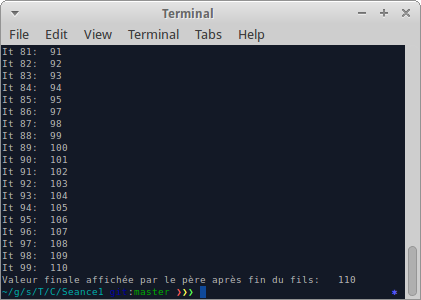
\includegraphics[width=0.66\textwidth]{seance2_img1.png}
  \caption{Sortie du programme}
\end{figure}

On constate qu'à chaque itération du père, la valeur lue sur le segment partagée ne correspond pas au numéro de l'itération. Cela s'explique par le fait que l'exécution du père peut être interrompue par le CPU pour laisser le fils s'exécuter. Or le fils incrémente lui aussi cet entier partagé. Lorsque le fils et le père ont fini des s'exécuter, après les deux itérations de 100 tours donc, le père affiche la valeur de l'entier partagé. \textbf{On constate ici le problème : l'entier devrait valoir 200 (100*2 incrémentations) or ce n'est jamais le cas.}

\section{Ajout d'un sémaphore}

La solution à ce problème est d'ajouter un sémaphore d'exclusion mutuelle (qui vaut 1). Avant chaque accès à la zone critique (lecture) et jusqu'à l'écriture du nouvel entier partagé, on décremente le sémaphore (cela bloque donc les autres processus qui faire la même chose). Après l'écriture du nouvel entier partagé, on l'incrémente à nouveau de 1. Ainsi les autres processus peuvent à leur tour décrémenter le sémaphore et modifier l'entier partagé, et ainsi de suite.

\subsection{Code corrigé}

\textcode{excl-mutu.c}
\begin{lstlisting}
...
void afaire(int isFather) {
    int j;
    for (j = 0; j<100;j++) {
        P(0); // Début de zone critique
        // Incrémentation de l'entier partagé grâce à la variable locale
        V(0); // Fin de zone critique
        usleep((rand()%81) + 20);
        if (isFather == 1) printf("It %d:\t%d\n",j,*adr);
    }
}

int main() {
    ...
    init_semaphore();
    val_sem(0,1);
    switch (son = fork()) {
        case 0:
            ...
        case -1:
            ...
        default:
            ...
            detruire_semaphore();
    }
    return 0;
}
\end{lstlisting}

\subsection{Sortie du programme avec sémaphore}

On constate dans le screenshot ci-desous que la valeur finale de l'entier partagé est 200, ce qui est la valeur attendue. À chaque fois que le fils ou le père ont lu et modifié l'entier partagé, ils se sont exclus mutullement (bloqués). Ainsi, aucun processus ne pouvait modifier l'entier partagé alors que l'autre n'avait pas fini de le modifier.

\begin{figure}[h!]
  \centering
  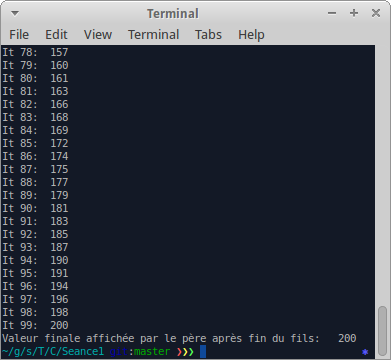
\includegraphics[width=0.66\textwidth]{seance2_img2.png}
  \caption{Sortie du programme}
\end{figure}

\chapter{Utilisation de la bibliothèque pour un producteur-consommateur}

Le but de cet exercice est de produire et consommer (par deux processus respectivement différents) des entiers contenus un tableau (en mémoire partagée) circulaire de taille 5. Le producteur doit s'arrêter quand le tableau est plein (et attendre qu'il y ait une place libre avant de le remplir à nouveau) et inversement pour le consommateur, il ne doit \og consommer\fg{} que s'il y a au moins une place occupée (donc si le tableau n'est pas vide). \textbf{Cela se met en \oe{}uvre grâce à deux sémaphores :}
\begin{itemize}
  \item Un sémaphore correspondra aux emplacements libres dans le tableau, il sera donc initialisé à 5 et sera décrémenté à chaque fois qu'un entier est produit
  \item Un sémaphore correspondra aux emplacement occupés dans le tableau, il sera donc initialisé à 0 et sera incrémenté à chaque fois qu'un entier est produit
\end{itemize}

\section{Rôles du consommateur et du producteur}
Par conséquent, le consommateur incrémentera le sémaphore des places libres et décrémentera celui des places occupées à chaque fois qu'il lira un entier. Le producteur fera l'inverse à chaque fois qu'il écrira un nouvel entier.

\medskip

Quand il n'y aura plus de place libre, le producteur se verra bloqué lorsqu'il essaiera de décrementer le sémaphore. De même, lorsqu'il n'y aura plus de place occupée, le consommmateur sera verra bloqué lorsqu'il essaiera de décrémenter le sémaphore. \textbf{Les contraintes du sujet de l'excercice sont donc respectées.}

\section{Index de lecture et d'écriture}

Un index \lstinline{int i} propre au consommateur et au producteur sera incrémenté à chaque fois que l'un ou l'autre produira ou consommera. De manière à avoir un tableau circulaire, cet index sera toujours \og lu\fg{} modulo 5.

\section{Code}

\textcode{prod-conso.c}
\begin{lstlisting}
#include <stdio.h>
#include <stdlib.h>
#include <sys/types.h>
#include <sys/ipc.h>
#include <sys/shm.h>
#include <unistd.h>

// CONSTANTES (noms des sémaphores)
int const SEM_PLACES_LIBRES = 0;
int const SEM_PLACES_OCCUPEES = 1;

int shmid;
int *adr;

int main() {
    int i;
    shmid = shmget(IPC_PRIVATE,5*sizeof(int),IPC_CREAT|IPC_EXCL|0666); // Création d'un espace de mémoire partagé de taille 5 entiers
    adr = (int*) shmat(shmid,NULL,0); // Shell memory attachment

    // Initialisations des 2 sémaphores avec leurs valeurs
    init_semaphore();
    val_sem(SEM_PLACES_LIBRES,5);
    val_sem(SEM_PLACES_OCCUPEES,0);

    srand(time(NULL));

    switch (fork()) {
        case 0:
            printf("%d Fils créé\n",getpid()); // producteur
            int tmp;
            for (i = 0; i<10; i++) { // On aurait pu faire un while(true)
                P(SEM_PLACES_LIBRES);
                tmp = (rand()%50) + 1;
                adr[i%5] = tmp;
                printf("Ajouté: %d\n",tmp);
                V(SEM_PLACES_OCCUPEES);
            }
            shmdt(adr); // détache le segment
            break;
        case -1:
            printf("Erreur\n");
            exit(0);
        default:
            printf("%d Père créé.\n",getpid()); // consommateur
            for (i = 0; i<10; i++) { // On aurait pu faire un while(true)
                P(SEM_PLACES_OCCUPEES);
                printf("Consommé: %d\n",adr[i%5]);
                V(SEM_PLACES_LIBRES);
            }
            shmdt(adr); // détache le segment
            shmctl(shmid,IPC_RMID,0); // Shell memory control : permet de supprimer la mémoire partagée
            detruire_semaphore();
    }
    return 0;
}
\end{lstlisting}

\section{Sortie du programme}

Voici la sortie du programme (ci-dessous). On constate que le fils produit les 5 entiers jusqu'à ce que le tableau soit plein, avant que le CPU ne laisse le père s'exécuter. On constate que l'ordre de création (production) des entiers correspond bien à l'ordre de lecture (consommation), les index fonctionnent donc bien. Enfin, chaque processus s'arrête si le tableau est vide ou plein : la contrainte est respectée.

\begin{figure}[h!]
  \centering
  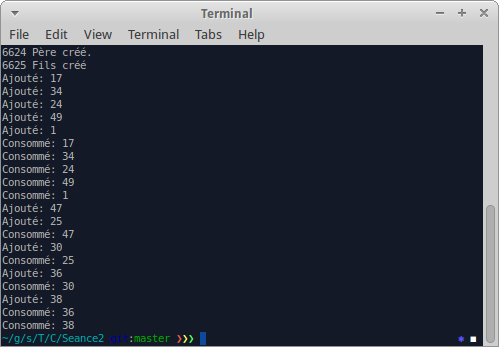
\includegraphics[width=0.66\textwidth]{seance2_img3.png}
  \caption{Sortie du programme}
\end{figure}

\end{document}
